%%%%%%%%%%%%%%%%%%%%%%%%%%%%%%%%%%%%%%%%%%%%%%%%%%%%%%%%%%%%%%%%%%%%%%%%%%%%%%%%
% Chapter 2: Conceptos
%%%%%%%%%%%%%%%%%%%%%%%%%%%%%%%%%%%%%%%%%%%%%%%%%%%%%%%%%%%%%%%%%%%%%%%%%%%%%%%%

%++++++++++++++++++++++++++++++++++++++++++++++++++++++++++++++++++++++++++++++
% \section{Navegación robótica}
% \label{2:sec:4}
% https://en.wikipedia.org/wiki/Mobile_robot_navigation
La navegación robótica es la habilidad que permite a un robot móvil poder
localizarse en el entorno y poder moverse libremente por el mismo, a partir del
conocimiento extraído de las imágenes obtenidas del medio. El objetivo principal
es conocer por donde debe y no debe navegar con la idea de poder alcanzar un
punto de destino marcado previamente. 

En la robótica móvil es indispensable saber como moverse por el mundo, además de
conocer que situaciones de riesgo se han de evitar: colisiones, superficies
irregulares, zonas prohibidas, etc. 

Es posible subdividir la navegación dependiendo de la zona de estudio: de
interiores o de exteriores. En ambos casos las tecnologías pueden ser las
mismas, sin embargo mientras que en la localización en exteriores se suele hacer
uso de GPS, odometría mecánica, etc., en interiores es posible conseguir mejores
resultados con sensores ópticos como cámaras, odometría láser, etc.

La navegación robótica se caracteriza por estos tres tópicos:

\begin{itemize}
  \item \textbf{Localización:} localizarse en el entorno. 
  \item \textbf{Búsqueda de caminos:} búsqueda del camino más optimo para llegar
  a un objetivo. 
  \item \textbf{Mapeo robótico:} construcción de un mapa del entorno. 
\end{itemize}% nube de puntos

%--------------------------------------
\subsection{Localización}
% http://www-math.mit.edu/~hajiagha/cars-fof.pdf
% http://ieeexplore.ieee.org/xpl/login.jsp?tp=&arnumber=1241767&url=http%3A%2F%2Fieeexplore.ieee.org%2Fxpls%2Fabs_all.jsp%3Farnumber%3D1241767

La localización es el primer tema a abordar en la navegación de un robot. El
objetivo es dar respuesta al '¿dónde estoy?', a través de conocer la posición
inicial, conocer la posición del punto de destino y autolocalizarse por el
entorno. La localización se puede dividir en dos grupos principales: basada en
puntos de referencias y basada en el análisis de las imágenes.

La localización basada en puntos de referencias se aprovecha en los puntos de
referencias que existen en el entorno y sobresalen de las imágenes de la escena
sin verse influenciados por otros factores de las escenas como los cambios en el
entorno o de los elementos que lo componen. Este tipo de puntos o marcas pueden
ser artificiales (líneas o flechas en un mapa o GPS) o naturales (puertas,
esquinas, senderos, etc.).

\begin{figure}[!th]
  \begin{center}
    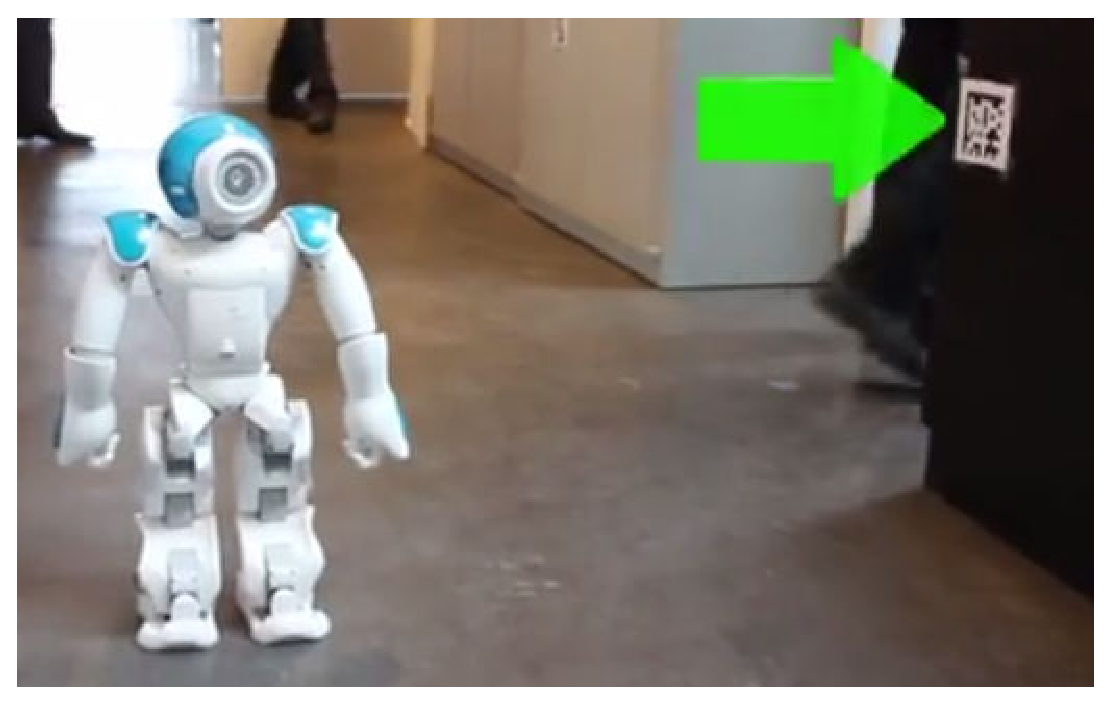
\includegraphics[width=0.5\textwidth]{images/cap2/LocalizacionMarcas.eps}
    \caption{Localización a través de código QR}
    \label{fig:LocalizacionMarcas}
  \end{center}
\end{figure}

Cuando este tipo de marcas no se pueden separar de las imágenes, porque bien no
se tienen puntos de referencia artificiales, o no se puede reconocer del propio
entorno marcas artificiales, se recurre a la localización basada en el análisis
de las imágenes capturadas. El primer paso es el 'autro-aprendizaje',
habitualmente navegar de forma autónoma y recoger las imágenes del entorno.
Estas imágenes se procesan, comparando los elementos en la escena de cada nueva
imagen recogida con la anterior y las imágenes que se tiene en el histórico,
obteniendo así la localización actual.

\begin{figure}[!th]
  \begin{center}
    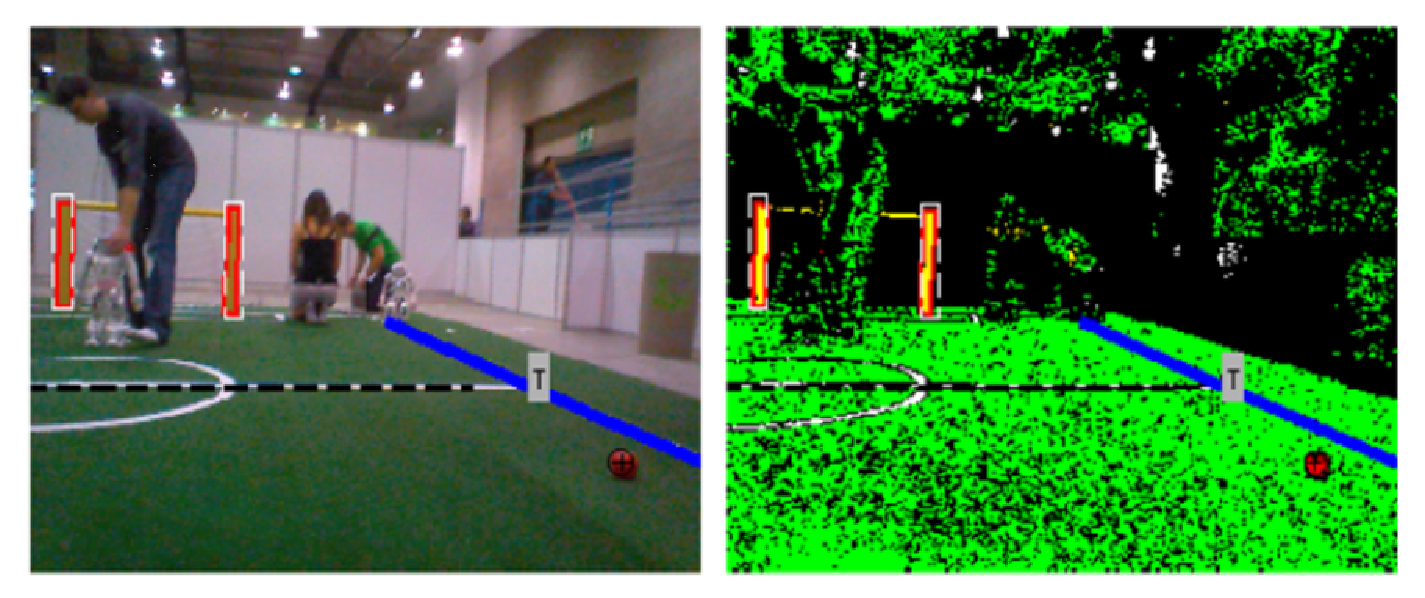
\includegraphics[width=0.5\textwidth]{images/cap2/LocalizacionImagenes.eps}
    \caption{Localización mediante los elementos de la escena}
    \label{fig:LocalizacionImagenes}
  \end{center}
\end{figure}

%--------------------------------------
\subsection{Búsqueda de caminos}
% https://en.wikipedia.org/wiki/Motion_planning
% http://correll.cs.colorado.edu/?p=965
% http://ais.informatik.uni-freiburg.de/teaching/ss11/robotics/slides/18-robot-motion-planning.pdf
% http://rabida.uhu.es/dspace/bitstream/handle/10272/5501/Nuevas_aportaciones_en_algoritmos_de_planificacion.pdf?sequence=2
La búsqueda de caminos permite hallar el conjunto de movimientos que permite a
un robot encontrar el camino más óptico hasta llegar a su objetivo, para no
solamente llegar en el menor tiempo posible, sino también evitar por el camino
los obstáculos que hagan peligrar el estado del robot o simplemente le retrasen.

El problema de la búsqueda de caminos ha sido ampliamente estudiado, existiendo
múltiples algoritmos para solventar este problema. 

Entre los métodos más conocidos están los 'roadmap', los cuales se basan en
construir una descripción de todo el espacio libre en el plano mediante un
grafo. Posteriormente los nodos del grafo se van conectando a partir de las
distancias más cortas entre sí, formando todos los caminos posibles, entre los
que se encuentra el más óptimo.

\begin{figure}[!th]
  \begin{center}
    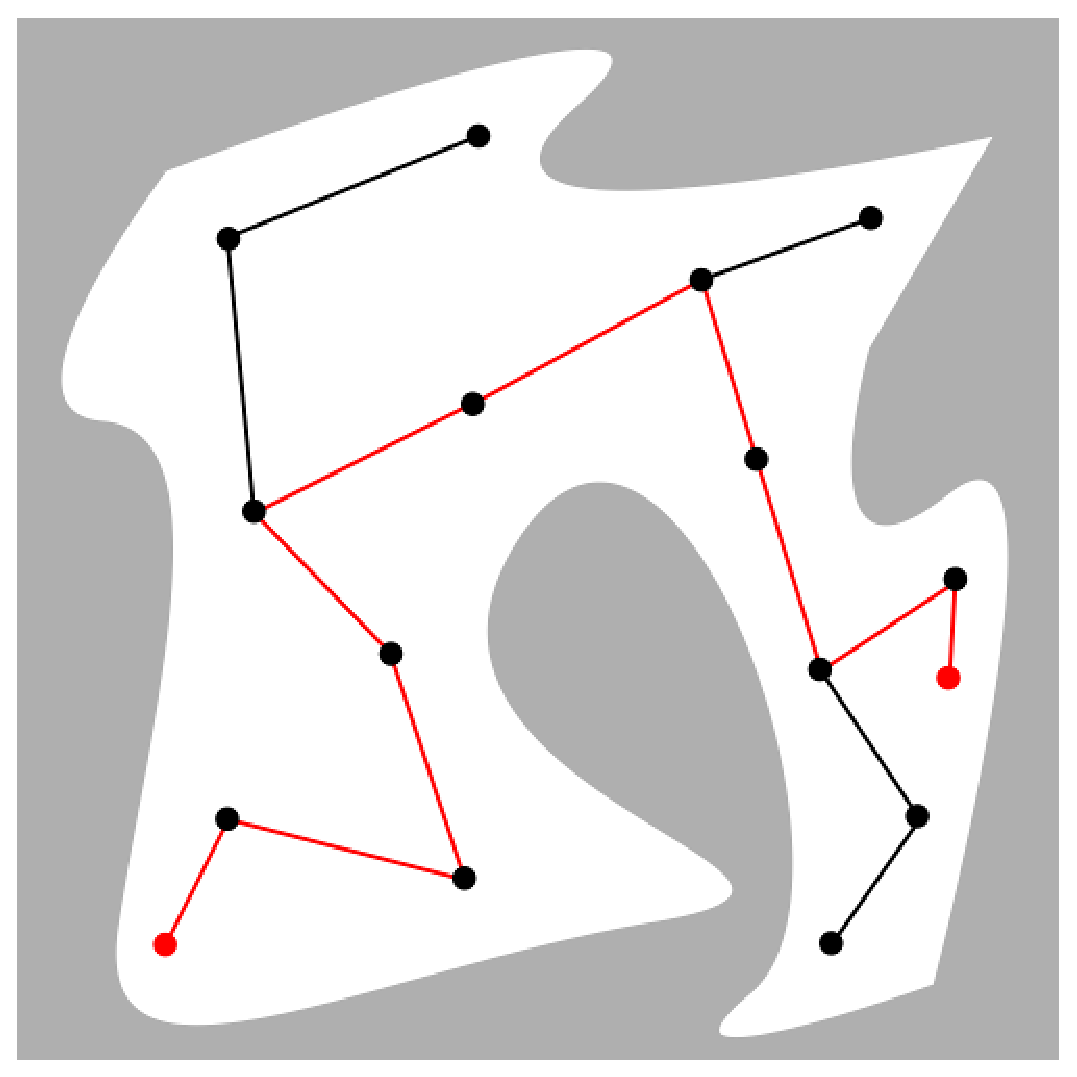
\includegraphics[width=0.5\textwidth]{images/cap2/BusquedaCaminosRoadmap.eps}
    \caption{Ejemplo de un 'roadmap'}
    \label{fig:BusquedaCaminosRoadmap}
  \end{center}
\end{figure}

Por otra parte, existen los métodos de descomposición en celdas, que en vez de
representar el entorno en un grafo, dividen el espacio libre de colisiones en un
conjunto de celdas. 

En los ultimos años han surgido métodos alternativos que permiten dar solución a
la complejidad del entornos y las restricciones cinemáticas que puede presentar
un robot en la búsqueda de caminos, son los algoritmos de generación aleatoria,
el más famoso es el RRT o 'Rapidly Exploring Random Trees', muy utilizados en la
navegación autónoma. Este algoritmo se basa en la construcción al azar de un 
árbol que va creciendode manera incremental mediante la captura de nuevas
muestras del entorno.

%--------------------------------------
\subsection{Mapeo robótico}
% https://en.wikipedia.org/wiki/Robotic_mapping
% https://en.wikipedia.org/wiki/3D_reconstruction_from_multiple_images
% Introduccion sobre el mapeo en robotica, que es porque...

El mapeo robótico 

%--------------------------------------
% \subsection{SLAM} dentro de mapeo...


%++++++++++++++++++++++++++++++++++++++++++++++++++++++++++++++++++++++++++++++
